\documentclass[10pt,a4paper]{article}
\usepackage[utf8]{inputenc}
\usepackage{amsmath}
\usepackage{amsfonts}
\usepackage{amssymb}
\usepackage{graphicx} 
\usepackage{float}
\usepackage{verbatim}
\begin{document}


\section{Rete neurale}
\label{Rete neurale}

Durante il periodo 24/05 - 31/05 mi sono occupata dello sviluppo di una Rete neurale in grado di ricevere in input un training set di dimensione 6 e di restituire una previsione sui dati di apprendimento ricevuti.
\noindent
Il problema trattato dalla rete \`e quello discusso nel precedente documento \textit{Analisi dei dati di probabilit\`a}
\\\\
Per aggevolare l'apprendimento della rete, ed ottenere delle previsioni stabili mi sono occupata di implementare due metodi di generazione randomica di dati in modo da far apprendere massiciamente la stessa.
Il dato prodotto consiste in un vettore di 6 elementi, composto da 0, 1 e -1 con il seguente criterio:
\begin{itemize}
\item \textbf{-1}: la domanda x non \`e stata posta al candidato;
\item \textbf{0}: la domanda x \`e stata posta al candidato che ha risposto in maniera errata;
\item \textbf{1}: la domanda x \`e stata posta al candidato che ha saputo rispondere correttamente.
\end{itemize}
\noindent
Il primo metodo che ho sviluppato si occupa di generare un vettore di dati di apprendimento basandosi esclusivamente su come le domande sono interconnesse tra di loro (grazie all'uso di un grafo della conoscenza costruito ad hoc); il secondo metodo ripropone quanto perseguito dal primo metodo con il valore aggiunto di generazione di un profilo randomico di un candidato, che tiene conto della risposta ad una domande seguendo la formula P(A)= $\frac{1}{3}+\frac{1}{6}P(S_1)+\frac{2}{3}P(S_2)$.

\subsection{Configurazione della Rete}
\label{Configurazione della Rete}

Configurazione della rete utilizzata:\\
\begin{verbatim}layer_defs = [];
layer_defs.push({type:'input', out_sx:1, out_sy:1, out_depth:6});
layer_defs.push({type:'fc', num_neurons:4, activation: 'tanh'});
layer_defs.push({type:'fc', num_neurons:4, activation: 'tanh'});
layer_defs.push({type:'regression', num_neurons:6});

net = new convnetjs.Net();
net.makeLayers(layer_defs);

trainer = new convnetjs.SGDTrainer(net, {learning_rate:0.01,
 momentum:0.1, batch_size:10, l2_decay:0.001});
\end{verbatim}
\noindent
I layer utilizzati sono due e compositi da 4 neuroni ciascuno vista la numerosit\`a dei dati di training che ho impiegato durante l'addestramento, in modo che alla rete risulti possibile imparare in modo adeguato. Attenzione se la rete presentasse un numero d neuroni troppo elevato la previsione ritornerebbe l'identit\`a del vettore di input della stessa, come conseguenza diretta della capacit\`a troppo elevata di immagazzinare dati.\\
Il numero di neuroni in regressione devono essere 6, perch\`e l'output che ci si aspetta da un vettore di dimensione \`e composto da 6 elementi.
\noindent
Per costruire un dataset di dati consistente che permettesse alla rete di imparare qualcosa ho costruito un grafo con lo scopo di mettere relazione degli argomenti che coinvolgono uno o pi\`u domande.
\begin{figure}[H]
\centering
	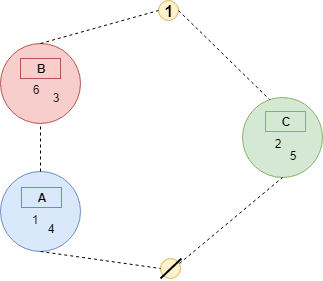
\includegraphics[width=0.60\linewidth]{image/grafo_trainset.png}
	\caption{Grafo presentante le relazioni esistenti tra il set di domande di prova.}
\end{figure}
\noindent
Per svolgere l'apprendimento ogni vettore, facente parte del dataset, viene dato in pasto alla rete che a sua volta provvede alla sua assimilazione come conoscenza mediante la tecnica dell'autoencoder,
ovvero la rete impara il vettore riducendone lo spazio occupato.
Per creare il dataset sono generati \textit{2000} vettori di risposta in modo che sia possibile compiere in maniera esaustivo l'apprendimento della rete.
\\
Il vettore passato in input per svolgere le previsioni \`e \textit{[0,1,0,0,0,0]}. 
Di seguito riporto quanto \`e stato rilevato in  fase di test.
\noindent

\subsection{Osservazioni riscontrate}
\label{Osservazioni riscontrate}

\subsubsection{Training set standard}
\label{Training set standard}
\begin{itemize}
\item \begin{verbatim}[-0.016830235758319205,0.11373169602342478,-0.17021775447616036,
-0.3011057468668946,0.04483733342756383,0.030344506696399966] \end{verbatim}
Appaiono in relazione le domande 1, 4, 3 e 2, 5 ,6.\\
Gli scostamenti tra le coppie 1 e 4, 2 e 5 sono consistenti con quelle che sono le relazioni  di dipendenza fra le domande, invece per quanto concerne la coppia 3 e 6 sono dovuti dalla presenza di -1  all'interno dei vettori di training.
Le domande 3 e 6 si dovrebbero presentare con una positivit\`a inferiore rispetto a 1 e 4; nel test in analisi questo vale per la domanda 4, la domanda 6 si presenta non conforme a tale regola, da ricondurre alla bont\`a del vettore di training.

\item \begin{verbatim}[-0.11235743604300916,-0.39879459369010783,-0.6219582601088702,
0.22754749414916,-0.3307584554090044,-0.39007701490038627] \end{verbatim}\\
Appaiono in relazione le domande 1, 2, 3, 5, 6 e 4.\\
Gli scostamenti tra le coppie 3 e 6, 2 e 5 sono consistenti con quelle che sono le relazioni di dipendenza fra le domande, invece per quanto concerne la coppia 1 e 4 sono dovuti dalla presenza di -1  all'interno dei vettori di training.
Le domande 3 e 6 si dovrebbero presentare con una positivit\`a inferiore rispetto a 1 e 4; nel test in analisi sia la domanda 1 che 4 si presentano conformi alla regola.

\item \begin{verbatim}[0.03741081925267472,-0.41568480234019844,-0.04549405829634745,
0.017658192512607442,0.30368782942992884,-0.5175456036018117] \end{verbatim}\\
Appaiono in relazione le domande 1, 4, 5 e 2, 3 e 6.\\
Gli scostamenti tra le coppie 1 e 4, 3 e 6 sono consistenti con quelle che sono le relazioni di dipendenza fra le domande, invece per quanto concerne la coppia 2 e 5 sono dovuti alla presenza di -1 all'interno dei vettori di training.
Le domande 3 e 6 si dovrebbero presentare con una positivit\`a inferiore rispetto a 1 e 4; nel test in analisi la domanda 1 che 4 si presentano conformi alla regola.

\item \begin{verbatim}[0.21422605841447054,-0.2636944179712092,-0.3706563171790509
,0.7764017490883244,-0.23816083562639187,-0.2524885890953481]\end{verbatim}
Appaiono in relazione 1, 4 e 2, 3, 5, 6.\\
Gli scostamenti tra le coppie  1 e 4, 2 e 5, 3 e 6 sono consistenti con quelle che sono le relazioni di dipendenza fra le domanda.
Le domande 3 e 6 si dovrebbero presentare con una positivit\`a inferiore rispetto a 1 e 4 ;nel test in analisi tale regola viene rispettata perfettamente

\end{itemize}


\subsubsection{Training set con generazione del profilo di un candidato e calcolo delle probabilit\`a di risposta}
\begin{itemize}

\item \begin{verbatim}[0.16367607727167577,-0.32053744790295396,-0.40842903200021335,
-0.06582359394312984,0.07811426051161906,0.4328108062656628] \end{verbatim}\\
Appaiono in relazione le domande 1, 5 , 6 e 2, 3, 4.\\
Le domanda 1 e 4, 3 e 6, 2 e 5 non sono pi\`u in relazione stretta. La domanda 1 e 4 si presenta con una positivit\`a inferiore rispetto alla domanda 6. Questo \`e causato dall'uso di un set con dati "spuri" calcolati mediante la probabilit\`a che un candidato ha di rispondere correttamente o meno ad una i-esima domanda, tale formula ha fatto venire meno la validit\`a parziale delle relazioni che intercorrono tra le domande.


\item \begin{verbatim}[0.18433537518873258,-0.04044612583630426,0.2352140436212822,
0.6613310411084423,-0.09050917524592572,-0.18953180536551828] \end{verbatim}\\
Appaiono in relazione le domande 1, 3, 4 e 2, 5, 6.\\
Le domande 1, 4 e 2, 5 sono in relazione fra di loro, questo non accade per le domande 3 e 6. La domanda 1 ha una positivit\`a inferiore alla domanda 3. Tali scostamenti tra le relazioni delle domande \`e dovuto all'uso di un set di dati con dati "spuri".

\item \begin{verbatim}[0.2549870388727452,-0.10818305932044818,-0.17180484931757034,
-0.1499695031382972,0.13676901446678133,-0.08494828483661017] \end{verbatim}\\
Appaiono in relazione le domande 1, 5 e 2, 3, 4, 6.
Le domande 3 e 6 rimangono in relazione tra di loro, cosa che non accede per le coppie 1, 4 e 2 e 5. La domanda 4 ha una positivit\`a inferiore rispetto alla domanda 6.  Tali scostamenti tra le relazioni delle domande \`e dovuto all'uso di un set di dati con dati "spuri".

\item \begin{verbatim}[-0.33701211585938906,0.7486270484471413,0.3102856894524609,
-0.0636999660997703,-0.30970127841579165,-0.03340342213139264] \end{verbatim}\\
Appaiono in relazione le domande 1, 4, 5, 6 e 2, 3.\\
Le domande 1 e 4 rimangono in relazione tra di loro, cosa che non accade per le domande 3, 6 e 2, 5. La domanda 1 ha una positivi\`a inferiore rispetto alla domanda 6 e 3, la domanda 4 invece si presenta con una positivit\`a inferiore sia alla domanda 3 che alla domanda 6. Tali scostamenti tra le relazioni delle domande \`e dovuto sempre dall'uso di un set di dati con dati "spuri".

\end{itemize}



\end{document}